% SMA-1 Figure 1 -- System overview (4 dense panels a-d)
% Conceptual / schematic only. NO numbers, accuracies, bars, radars.
% Caption is supplied by the manuscript LaTeX, NOT baked here.
\documentclass[border=4pt]{standalone}
\usepackage{amsmath}
\usepackage{amssymb}
\usepackage{pifont}
\usepackage{fontspec}
\setsansfont{Arimo}
\renewcommand{\familydefault}{\sfdefault}
\usepackage{tikz}
\usetikzlibrary{arrows.meta,positioning,calc,fit,backgrounds,shapes.geometric,shapes.symbols,decorations.pathreplacing,decorations.pathmorphing,patterns}

% ---- Design palette (SMA-1 NMI figure system) ----
\definecolor{ink}{HTML}{1A1C1E}       % primary ink
\definecolor{ink7}{HTML}{3D4248}      % strong secondary
\definecolor{ink5}{HTML}{6B7177}      % secondary labels
\definecolor{ink4}{HTML}{8A9097}      % tertiary / baseline gray
\definecolor{ink3}{HTML}{B4B9BE}      % light strokes
\definecolor{ink2}{HTML}{D6D9DC}      % hairlines
\definecolor{ink1}{HTML}{EAECEE}      % neutral fill
\definecolor{ink05}{HTML}{F4F5F6}     % panel tint
\definecolor{titlegray}{HTML}{565C62}
% semantic accents
\definecolor{teal}{HTML}{3F8A83}      % method / SMA
\definecolor{teal2}{HTML}{4FA89F}     % active path
\definecolor{tealtint}{HTML}{E6F0EF}
\definecolor{amber}{HTML}{C2883C}     % warning / information content
\definecolor{ambertint}{HTML}{F6ECDD}
\definecolor{redf}{HTML}{C05A50}      % failure / novelty
\definecolor{redtint}{HTML}{F6E2E0}
\definecolor{greenk}{HTML}{3E9B63}    % kept / normal
\definecolor{greentint}{HTML}{E2F0E8}
% lattice + first/higher order
\definecolor{fo}{HTML}{5AA9C4}        % first-order functor
\definecolor{ho}{HTML}{2E6B86}        % higher-order relation
\definecolor{vio}{HTML}{9B86C4}       % lattice ascension violet
\definecolor{viotint}{HTML}{ECE6F4}
% baselines
\definecolor{kggold}{HTML}{E2A85B}    % knowledge-graph gold
\definecolor{kggold2}{HTML}{C68A2E}
% domain accents
\definecolor{dmed}{HTML}{C0504D}
\definecolor{dgen}{HTML}{3E8E5A}
\definecolor{dcyb}{HTML}{4A6F8A}
\definecolor{dleg}{HTML}{7A5DA8}
\definecolor{dfin}{HTML}{C68A2E}
\definecolor{dche}{HTML}{2E8AA6}

\begin{document}
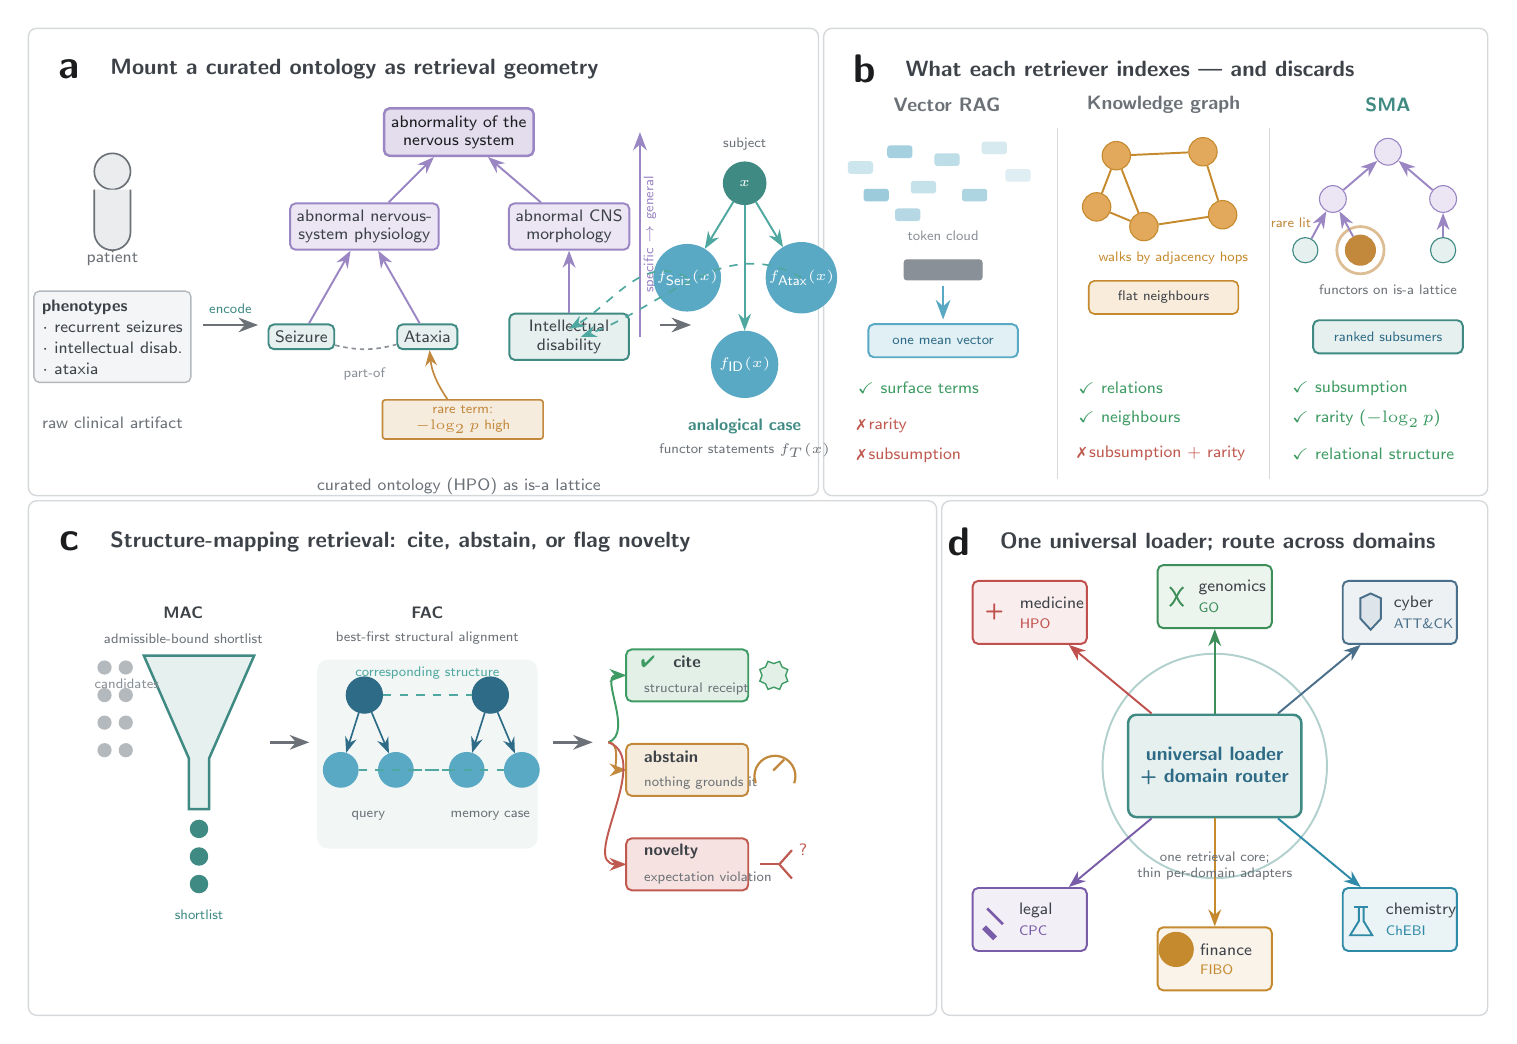
\begin{tikzpicture}[
  font=\sffamily,
  >=Stealth,
  pletter/.style={font=\sffamily\bfseries\Large, color=ink},
  ptitle/.style={font=\sffamily\bfseries\footnotesize, color=ink7, align=left},
  psub/.style={font=\sffamily\fontsize{6.4}{7.4}\selectfont, color=ink5, align=left},
  lab/.style={font=\sffamily\fontsize{6.6}{7.8}\selectfont, color=ink7, align=center},
  smalllab/.style={font=\sffamily\fontsize{5.8}{6.8}\selectfont, color=ink5, align=center},
  tinylab/.style={font=\sffamily\fontsize{5.2}{6}\selectfont, color=ink5, align=center},
  mono/.style={font=\ttfamily\fontsize{6}{7}\selectfont, color=ink7},
  panelbg/.style={draw=ink2, line width=0.5pt, fill=white, rounded corners=3pt},
  divider/.style={draw=ink2, line width=0.4pt},
  % nodes
  cnode/.style={circle, draw=teal, fill=teal, text=white, font=\sffamily\fontsize{5.2}{5.8}\selectfont, inner sep=0.5pt, minimum size=5mm, align=center},
  fnode/.style={circle, draw=fo, fill=fo, text=white, font=\sffamily\fontsize{5}{5.6}\selectfont, inner sep=0.5pt, minimum size=5mm, align=center},
  hnode/.style={circle, draw=ho, fill=ho, text=white, font=\sffamily\fontsize{5}{5.6}\selectfont, inner sep=0.5pt, minimum size=5.4mm, align=center},
  latnode/.style={rounded corners=2pt, draw=vio, line width=0.7pt, fill=viotint, text=ink7, font=\sffamily\fontsize{5.8}{6.6}\selectfont, inner sep=2.4pt, align=center},
  latroot/.style={rounded corners=2pt, draw=vio, line width=0.9pt, fill=vio!28, text=ink, font=\sffamily\fontsize{5.8}{6.6}\selectfont, inner sep=2.6pt, align=center},
  isa/.style={->, line width=0.7pt, color=vio},
  partof/.style={-, dashed, line width=0.6pt, color=ink4, dash pattern=on 1.6pt off 1.4pt},
  ftateal/.style={->, line width=0.7pt, color=teal2},
  flow/.style={->, line width=0.9pt, color=ink5},
  keep/.style={font=\sffamily\fontsize{5.6}{7.2}\selectfont, color=greenk, align=left},
  disc/.style={font=\sffamily\fontsize{5.6}{7.2}\selectfont, color=redf, align=left},
]

% ===================================================================
% Overall: 4 panels. Top row a (wide) + b. Bottom row c (wide) + d.
% Canvas approx 18.2 wide x 12.4 tall.
% ===================================================================

% ----- panel frames -----
\begin{scope}[on background layer]
  \node[panelbg, fit={(-0.25,6.55) (9.55,12.25)}] (Pa) {};
  \node[panelbg, fit={(9.85,6.55) (18.05,12.25)}] (Pb) {};
  \node[panelbg, fit={(-0.25,-0.05) (11.05,6.25)}] (Pc) {};
  \node[panelbg, fit={(11.35,-0.05) (18.05,6.25)}] (Pd) {};
\end{scope}

% ========================== PANEL A ==========================
% Mount a curated ontology as retrieval geometry.
\node[pletter] at (0.15,11.85) {a};
\node[ptitle] at (0.55,11.85) [anchor=west] {Mount a curated ontology as retrieval geometry};

% --- raw clinical artifact (left) ---
\begin{scope}[shift={(0.15,7.0)}]
  % patient glyph
  \node[circle, draw=ink5, fill=ink1, line width=0.6pt, minimum size=4.6mm, inner sep=0pt] (phead) at (0.55,3.55) {};
  \draw[ink5, line width=0.6pt, fill=ink1] (0.32,3.32) -- (0.32,2.78) arc (180:360:0.23) -- (0.78,3.32);
  \node[smalllab, anchor=north] at (0.55,2.66) {patient};
  % phenotype list card
  \node[draw=ink3, fill=ink05, rounded corners=2pt, line width=0.5pt, align=left,
        inner sep=3pt, font=\sffamily\fontsize{5.8}{7.6}\selectfont, text=ink7] (card) at (0.55,1.45)
        {\textbf{phenotypes}\\$\cdot$ recurrent seizures\\$\cdot$ intellectual disab.\\$\cdot$ ataxia};
  \node[smalllab, anchor=north] at (0.55,0.55) {raw clinical artifact};
\end{scope}

% encode arrow A1
\draw[flow] (1.85,8.6) -- (2.55,8.6);
\node[tinylab, color=teal, anchor=south] at (2.2,8.62) {encode};

% --- is-a lattice (center) : 3 levels ---
\begin{scope}[shift={(2.55,7.0)}]
  % root
  \node[latroot] (root) at (2.55,4.05) {abnormality of the\\nervous system};
  % mid level
  \node[latnode] (mphys) at (1.35,2.85) {abnormal nervous-\\system physiology};
  \node[latnode] (mmorph) at (3.95,2.85) {abnormal CNS\\morphology};
  % leaf level (specific HPO terms)
  \node[latnode, draw=teal, fill=tealtint] (seiz) at (0.55,1.45) {Seizure};
  \node[latnode, draw=teal, fill=tealtint] (ataxia) at (2.15,1.45) {Ataxia};
  \node[latnode, draw=teal, fill=tealtint, text width=1.35cm] (id) at (3.95,1.45) {Intellectual\\disability};
  % is-a edges (solid, arrow toward general)
  \draw[isa] (mphys) -- (root);
  \draw[isa] (mmorph) -- (root);
  \draw[isa] (seiz) -- (mphys);
  \draw[isa] (ataxia) -- (mphys);
  \draw[isa] (id) -- (mmorph);
  % typed-relation edge (part-of, dashed)
  \draw[partof] (seiz) to[bend right=14] (ataxia);
  \node[tinylab, color=ink4] at (1.35,0.98) {part-of};
  % IC weight glyph on the rare/decisive term: Ataxia is the rare, decisive term.
  \node[draw=amber, fill=ambertint, line width=0.6pt, rounded corners=1pt,
        font=\sffamily\fontsize{5}{5.8}\selectfont, text=amber, inner sep=2pt, text width=1.9cm, align=center] (ic) at (2.6,0.4) {rare term: $-\!\log_2 p$ high};
  \draw[->, line width=0.6pt, color=amber] (ic) to[bend left=14] (ataxia);
  % ascension annotation
  \node[tinylab, color=vio, rotate=90, anchor=south] at (5.18,2.75) {specific $\to$ general};
  \draw[->, line width=0.8pt, color=vio] (4.85,1.45) -- (4.85,4.05);
\end{scope}
\node[smalllab, anchor=north] at (5.1,6.78) {curated ontology (HPO) as is-a lattice};

% encode arrow A2 -> analogical case
\draw[flow] (7.65,8.6) -- (8.05,8.6);

% --- analogical case (right) : functor statements ---
\begin{scope}[shift={(7.95,7.35)}]
  \node[cnode, minimum size=5.4mm] (x) at (0.78,3.05) {$x$};
  \node[tinylab, color=ink5, anchor=south] at (0.78,3.35) {subject};
  \node[fnode, minimum size=8.4mm, font=\sffamily\fontsize{4.6}{5.2}\selectfont] (fseiz) at (0.05,1.85) {$f_{\text{Seiz}}(x)$};
  \node[fnode, minimum size=8.4mm, font=\sffamily\fontsize{4.6}{5.2}\selectfont] (fatax) at (1.5,1.85) {$f_{\text{Atax}}(x)$};
  \node[fnode, minimum size=8.4mm, font=\sffamily\fontsize{4.6}{5.2}\selectfont] (fid) at (0.78,0.75) {$f_{\text{ID}}(x)$};
  \draw[ftateal] (x) -- (fseiz);
  \draw[ftateal] (x) -- (fatax);
  \draw[ftateal] (x) -- (fid);
  \node[smalllab, anchor=north, text=teal] at (0.78,0.18) {\textbf{analogical case}};
  \node[tinylab, color=ink5, anchor=north] at (0.78,-0.12) {functor statements $f_T(x)$};
\end{scope}
% teal correspondence: case functors link back to matched lattice leaves
\draw[ftateal, dashed, line width=0.6pt] (8.0,9.2) to[out=150,in=30] (6.5,8.55);
\draw[ftateal, dashed, line width=0.6pt] (9.45,9.2) to[out=150,in=20] (6.65,8.45);

% ========================== PANEL B ==========================
% What each retriever indexes -- and discards.
\node[pletter] at (10.25,11.85) {b};
\node[ptitle] at (10.65,11.85) [anchor=west] {What each retriever indexes --- and discards};

% three lanes
\begin{scope}[shift={(9.85,6.55)}]
  % lane separators
  \draw[divider] (2.85,0.1) -- (2.85,4.55);
  \draw[divider] (5.55,0.1) -- (5.55,4.55);

  % ---------- Lane 1: Vector RAG ----------
  \node[ptitle, font=\sffamily\bfseries\fontsize{6.6}{7.6}\selectfont, color=ink5] at (1.45,4.85) {Vector RAG};
  % token cloud collapsing into one vector
  \foreach \tx/\ty/\op in {0.35/4.05/30, 0.85/4.25/55, 1.45/4.15/40, 2.05/4.3/25, 0.55/3.7/60, 1.15/3.8/35, 1.8/3.7/50, 2.35/3.95/20, 0.95/3.45/45} {
    \node[fill=fo!\op, rounded corners=1pt, minimum width=3.2mm, minimum height=1.6mm, inner sep=0pt] at (\tx,\ty) {};
  }
  \node[tinylab, color=ink4] at (1.4,3.18) {token cloud};
  % rarity washed out chip
  \node[draw=ink3, fill=ink1, rounded corners=1pt, font=\sffamily\fontsize{4.8}{5.4}\selectfont, color=ink4, inner sep=1.4pt] at (1.4,2.75) {rarity faded};
  \draw[flow, color=fo] (1.4,2.55) -- (1.4,2.12);
  % one mean vector
  \node[draw=fo, fill=fo!18, rounded corners=2pt, line width=0.7pt, minimum width=1.9cm, minimum height=4.2mm, font=\sffamily\fontsize{5.4}{6}\selectfont, text=ho] at (1.4,1.85) {one mean vector};
  % keeps/discards
  \node[keep, anchor=west] at (0.18,1.25) {\checkmark{} surface terms};
  \node[disc, anchor=west] at (0.18,0.78) {\ding{55}\,rarity};
  \node[disc, anchor=west] at (0.18,0.40) {\ding{55}\,subsumption};

  % ---------- Lane 2: Knowledge graph ----------
  \node[ptitle, font=\sffamily\bfseries\fontsize{6.6}{7.6}\selectfont, color=ink5] at (4.2,4.85) {Knowledge graph};
  % node-edge graph with adjacency hops
  \node[circle, draw=kggold2, fill=kggold, minimum size=3.6mm, inner sep=0pt] (g1) at (3.6,4.2) {};
  \node[circle, draw=kggold2, fill=kggold, minimum size=3.6mm, inner sep=0pt] (g2) at (4.7,4.25) {};
  \node[circle, draw=kggold2, fill=kggold, minimum size=3.6mm, inner sep=0pt] (g3) at (4.95,3.45) {};
  \node[circle, draw=kggold2, fill=kggold, minimum size=3.6mm, inner sep=0pt] (g4) at (3.95,3.3) {};
  \node[circle, draw=kggold2, fill=kggold, minimum size=3.6mm, inner sep=0pt] (g5) at (3.35,3.55) {};
  \draw[-, line width=0.7pt, color=kggold2] (g1)--(g2) (g2)--(g3) (g3)--(g4) (g4)--(g5) (g5)--(g1) (g4)--(g1);
  \node[tinylab, color=kggold2, anchor=west] at (3.25,2.9) {walks by adjacency hops};
  \node[draw=kggold2, fill=kggold!22, rounded corners=2pt, line width=0.6pt, minimum width=1.9cm, minimum height=4.2mm, font=\sffamily\fontsize{5.4}{6}\selectfont, text=ink7] at (4.2,2.4) {flat neighbours};
  \node[keep, anchor=west] at (2.98,1.25) {\checkmark{} relations};
  \node[keep, anchor=west] at (2.98,0.86) {\checkmark{} neighbours};
  \node[disc, anchor=west] at (2.98,0.42) {\ding{55}\,subsumption + rarity};

  % ---------- Lane 3: SMA ----------
  \node[ptitle, font=\sffamily\bfseries\fontsize{6.6}{7.6}\selectfont, color=teal] at (7.05,4.85) {SMA};
  % functors on an is-a lattice with the rare-but-decisive node lit
  \node[circle, draw=vio, fill=viotint, minimum size=3.4mm, inner sep=0pt] (sroot) at (7.05,4.25) {};
  \node[circle, draw=vio, fill=viotint, minimum size=3.4mm, inner sep=0pt] (smid1) at (6.35,3.65) {};
  \node[circle, draw=vio, fill=viotint, minimum size=3.4mm, inner sep=0pt] (smid2) at (7.75,3.65) {};
  \node[circle, draw=teal, fill=tealtint, minimum size=3.2mm, inner sep=0pt] (sl1) at (6.0,3.0) {};
  % rare-but-decisive node LIT (amber halo)
  \node[circle, draw=amber, line width=1pt, fill=amber, minimum size=3.6mm, inner sep=0pt] (sl2) at (6.7,3.0) {};
  \begin{scope}[on background layer]\node[circle, draw=amber!55, line width=1pt, minimum size=6mm] at (6.7,3.0) {};\end{scope}
  \node[circle, draw=teal, fill=tealtint, minimum size=3.2mm, inner sep=0pt] (sl3) at (7.75,3.0) {};
  \draw[isa] (smid1) -- (sroot); \draw[isa] (smid2) -- (sroot);
  \draw[isa] (sl1) -- (smid1); \draw[isa] (sl2) -- (smid1); \draw[isa] (sl3) -- (smid2);
  \node[tinylab, color=amber, anchor=east] at (6.2,3.35) {rare lit};
  \node[tinylab, color=ink5] at (7.05,2.5) {functors on is-a lattice};
  \node[draw=teal, fill=tealtint, rounded corners=2pt, line width=0.7pt, minimum width=1.9cm, minimum height=4.2mm, font=\sffamily\fontsize{5.4}{6}\selectfont, text=ho] at (7.05,1.9) {ranked subsumers};
  \node[keep, anchor=west] at (5.7,1.25) {\checkmark{} subsumption};
  \node[keep, anchor=west] at (5.7,0.86) {\checkmark{} rarity ($-\!\log_2 p$)};
  \node[keep, anchor=west] at (5.7,0.42) {\checkmark{} relational structure};
\end{scope}

% ========================== PANEL C ==========================
% Structure-mapping retrieval: MAC -> FAC -> cite / abstain / novelty
\node[pletter] at (0.15,5.85) {c};
\node[ptitle] at (0.55,5.85) [anchor=west] {Structure-mapping retrieval: cite, abstain, or flag novelty};

\begin{scope}[shift={(0.15,0.0)}]
  % ---- MAC : funnel narrowing candidate set ----
  \node[smalllab, font=\sffamily\bfseries\fontsize{6.4}{7.4}\selectfont, color=ink7] at (1.45,4.95) {MAC};
  \node[tinylab, color=ink5] at (1.45,4.62) {admissible-bound shortlist};
  % candidate set (many) on the left of funnel
  \foreach \cy in {3.2,3.55,3.9,4.25} {
    \node[circle, fill=ink3, minimum size=1.8mm, inner sep=0pt] at (0.45,\cy) {};
    \node[circle, fill=ink3, minimum size=1.8mm, inner sep=0pt] at (0.72,\cy) {};
  }
  % funnel shape
  \draw[draw=teal, line width=0.8pt, fill=tealtint] (0.95,4.45) -- (2.35,4.45) -- (1.95,3.45) -- (2.35,2.55) -- (1.55,2.05) -- (0.95,2.55) -- cycle;
  % redraw a clean funnel (trapezoid -> neck)
  \begin{scope}
    \fill[white] (0.9,2.0) rectangle (2.45,4.55);
  \end{scope}
  \draw[draw=teal, line width=0.9pt, fill=tealtint]
        (0.95,4.4) -- (2.35,4.4) -- (1.78,3.1) -- (1.78,2.45) -- (1.52,2.45) -- (1.52,3.1) -- cycle;
  % shortlist (few) out the neck
  \node[circle, draw=teal, fill=teal, minimum size=2.2mm, inner sep=0pt] at (1.65,2.2) {};
  \node[circle, draw=teal, fill=teal, minimum size=2.2mm, inner sep=0pt] at (1.65,1.85) {};
  \node[circle, draw=teal, fill=teal, minimum size=2.2mm, inner sep=0pt] at (1.65,1.5) {};
  \node[tinylab, color=ink4, anchor=west] at (0.2,4.05) {candidates};
  \node[tinylab, color=teal, anchor=north] at (1.65,1.3) {shortlist};

  \draw[flow] (2.55,3.3) -- (3.05,3.3);

  % ---- FAC : two relational structures with dashed correspondences ----
  \node[smalllab, font=\sffamily\bfseries\fontsize{6.4}{7.4}\selectfont, color=ink7] at (4.55,4.95) {FAC};
  \node[tinylab, color=ink5] at (4.55,4.62) {best-first structural alignment};
  \begin{scope}[on background layer]\fill[teal!7, rounded corners=4pt] (3.15,1.95) rectangle (5.95,4.35);\end{scope}
  % left structure (query)
  \node[hnode, minimum size=4.6mm] (qh) at (3.75,3.9) {};
  \node[fnode, minimum size=4.4mm] (ql) at (3.45,2.95) {};
  \node[fnode, minimum size=4.4mm] (qr) at (4.15,2.95) {};
  \draw[->, line width=0.6pt, color=ho] (qh)--(ql); \draw[->, line width=0.6pt, color=ho] (qh)--(qr);
  \node[tinylab, color=ink5, anchor=north] at (3.8,2.55) {query};
  % right structure (memory case)
  \node[hnode, minimum size=4.6mm] (mh) at (5.35,3.9) {};
  \node[fnode, minimum size=4.4mm] (ml) at (5.05,2.95) {};
  \node[fnode, minimum size=4.4mm] (mr) at (5.75,2.95) {};
  \draw[->, line width=0.6pt, color=ho] (mh)--(ml); \draw[->, line width=0.6pt, color=ho] (mh)--(mr);
  \node[tinylab, color=ink5, anchor=north] at (5.35,2.55) {memory case};
  % correspondences (dashed teal)
  \draw[dashed, line width=0.7pt, color=teal2] (qh) -- (mh);
  \draw[dashed, line width=0.7pt, color=teal2] (ql) -- (ml);
  \draw[dashed, line width=0.7pt, color=teal2] (qr) -- (mr);
  \node[tinylab, color=teal2] at (4.55,4.18) {corresponding structure};

  \draw[flow] (6.15,3.3) -- (6.65,3.3);

  % ---- outcomes column : cite / abstain / novelty ----
  % cite (structural receipt / seal)
  \node[draw=greenk, fill=greentint, rounded corners=2pt, line width=0.7pt, minimum width=1.55cm, minimum height=6.6mm, align=center, font=\sffamily\fontsize{5.8}{6.6}\selectfont, text=ink7] (cite) at (7.85,4.15) {};
  \node[font=\sffamily\fontsize{6}{6.8}\selectfont, color=greenk] at (7.35,4.32) {\ding{52}};
  \node[smalllab, color=ink7, anchor=west] at (7.55,4.32) {\textbf{cite}};
  \node[tinylab, color=ink5, anchor=west] at (7.18,3.98) {structural receipt};
  % seal mark
  \node[star, star points=8, star point ratio=0.78, draw=greenk, fill=greentint, line width=0.5pt, minimum size=3mm, inner sep=0pt] at (8.95,4.15) {};

  % abstain (calibrated gauge)
  \node[draw=amber, fill=ambertint, rounded corners=2pt, line width=0.7pt, minimum width=1.55cm, minimum height=6.6mm, align=center, font=\sffamily\fontsize{5.8}{6.6}\selectfont, text=ink7] (abst) at (7.85,2.95) {};
  \node[smalllab, color=ink7, anchor=west] at (7.18,3.12) {\textbf{abstain}};
  \node[tinylab, color=ink5, anchor=west] at (7.18,2.78) {nothing grounds it};
  % gauge arc
  \draw[line width=0.8pt, color=amber] (8.72,2.78) arc (200:-20:0.26);
  \draw[line width=0.8pt, color=amber] (8.95,2.95) -- ++(0.13,0.13);
  \fill[amber] (8.95,2.95) circle (0.5pt);

  % flag novelty (expectation-violation fork)
  \node[draw=redf, fill=redtint, rounded corners=2pt, line width=0.7pt, minimum width=1.55cm, minimum height=6.6mm, align=center, font=\sffamily\fontsize{5.8}{6.6}\selectfont, text=ink7] (nov) at (7.85,1.75) {};
  \node[smalllab, color=ink7, anchor=west] at (7.18,1.92) {\textbf{novelty}};
  \node[tinylab, color=ink5, anchor=west] at (7.18,1.58) {expectation violation};
  % fork glyph
  \draw[line width=0.8pt, color=redf] (8.78,1.75) -- (9.02,1.75);
  \draw[line width=0.8pt, color=redf] (9.02,1.75) -- (9.18,1.93);
  \draw[line width=0.8pt, color=redf] (9.02,1.75) -- (9.18,1.57);
  \node[font=\sffamily\fontsize{5.6}{6}\selectfont, color=redf] at (9.32,1.93) {?};

  % branch arrows from FAC outcome to the three
  \draw[->, line width=0.7pt, color=greenk] (6.85,3.3) to[out=20,in=180] (7.08,4.15);
  \draw[->, line width=0.7pt, color=amber] (6.85,3.3) to[out=0,in=180] (7.08,2.95);
  \draw[->, line width=0.7pt, color=redf] (6.85,3.3) to[out=-20,in=180] (7.08,1.75);
\end{scope}

% ========================== PANEL D ==========================
% One universal loader; route across domains.
\node[pletter] at (11.45,5.85) {d};
\node[ptitle] at (11.85,5.85) [anchor=west] {One universal loader; route across domains};

\begin{scope}[shift={(11.35,-0.05)}]
  % concentric router ring (behind hub)
  \begin{scope}[on background layer]
    \node[circle, draw=teal!40, line width=0.7pt, minimum size=2.85cm] at (3.35,3.05) {};
  \end{scope}
  % central loader + router hub
  \node[draw=teal, fill=tealtint, line width=0.9pt, rounded corners=3pt,
        minimum width=2.2cm, minimum height=1.3cm, align=center, inner sep=3pt,
        text width=1.95cm, font=\sffamily\fontsize{6.8}{8}\selectfont, text=ho] (hub) at (3.35,3.05)
        {\textbf{universal loader}\\\textbf{+ domain router}};

  % six domain glyphs around the hub
  % positions: NW, N, NE, SW, S(used as SE), SE -> arrange 3 top, 3 bottom for clarity
  % medicine (top-left)
  \node[draw=dmed, fill=dmed!10, line width=0.7pt, rounded corners=2pt, minimum width=1.45cm, minimum height=8mm, align=center, font=\sffamily\fontsize{5.8}{6.6}\selectfont, text=ink7] (med) at (1.0,5.0) {};
  \node[font=\sffamily\bfseries\fontsize{8}{8}\selectfont, color=dmed] at (0.55,5.0) {+};
  \node[smalllab, color=ink7, anchor=west] at (0.75,5.12) {medicine};
  \node[tinylab, color=dmed, anchor=west] at (0.75,4.86) {HPO};

  % genomics (top-center)
  \node[draw=dgen, fill=dgen!10, line width=0.7pt, rounded corners=2pt, minimum width=1.45cm, minimum height=8mm, align=center, font=\sffamily\fontsize{5.8}{6.6}\selectfont, text=ink7] (gen) at (3.35,5.2) {};
  % helix glyph
  \draw[line width=0.7pt, color=dgen] (2.78,5.32) to[out=-40,in=140] (2.95,5.08);
  \draw[line width=0.7pt, color=dgen] (2.78,5.08) to[out=40,in=-140] (2.95,5.32);
  \node[smalllab, color=ink7, anchor=west] at (3.02,5.32) {genomics};
  \node[tinylab, color=dgen, anchor=west] at (3.02,5.06) {GO};

  % cyber (top-right)
  \node[draw=dcyb, fill=dcyb!10, line width=0.7pt, rounded corners=2pt, minimum width=1.45cm, minimum height=8mm, align=center, font=\sffamily\fontsize{5.8}{6.6}\selectfont, text=ink7] (cyb) at (5.7,5.0) {};
  % shield glyph
  \draw[line width=0.7pt, color=dcyb, fill=dcyb!18] (5.2,5.18) -- (5.2,4.92) -- (5.33,4.78) -- (5.46,4.92) -- (5.46,5.18) -- (5.33,5.24) -- cycle;
  \node[smalllab, color=ink7, anchor=west] at (5.5,5.12) {cyber};
  \node[tinylab, color=dcyb, anchor=west] at (5.5,4.86) {ATT\&CK};

  % legal (bottom-left)
  \node[draw=dleg, fill=dleg!10, line width=0.7pt, rounded corners=2pt, minimum width=1.45cm, minimum height=8mm, align=center, font=\sffamily\fontsize{5.8}{6.6}\selectfont, text=ink7] (leg) at (1.0,1.1) {};
  % gavel glyph
  \draw[line width=0.9pt, color=dleg] (0.46,1.24) -- (0.66,1.04);
  \draw[line width=2.0pt, color=dleg] (0.42,1.0) -- (0.56,0.86);
  \node[smalllab, color=ink7, anchor=west] at (0.74,1.22) {legal};
  \node[tinylab, color=dleg, anchor=west] at (0.74,0.96) {CPC};

  % finance (bottom-center)
  \node[draw=dfin, fill=dfin!10, line width=0.7pt, rounded corners=2pt, minimum width=1.45cm, minimum height=8mm, align=center, font=\sffamily\fontsize{5.8}{6.6}\selectfont, text=ink7] (fin) at (3.35,0.6) {};
  % coin glyph
  \node[circle, draw=dfin, line width=0.8pt, fill=dfin!18, minimum size=4.2mm, inner sep=0pt, font=\sffamily\fontsize{5}{5}\selectfont, color=dfin] at (2.86,0.72) {\$};
  \node[smalllab, color=ink7, anchor=west] at (3.04,0.72) {finance};
  \node[tinylab, color=dfin, anchor=west] at (3.04,0.46) {FIBO};

  % chemistry (bottom-right)
  \node[draw=dche, fill=dche!10, line width=0.7pt, rounded corners=2pt, minimum width=1.45cm, minimum height=8mm, align=center, font=\sffamily\fontsize{5.8}{6.6}\selectfont, text=ink7] (che) at (5.7,1.1) {};
  % flask glyph
  \draw[line width=0.7pt, color=dche] (5.18,1.26) -- (5.18,1.08) -- (5.07,0.9) -- (5.35,0.9) -- (5.24,1.08) -- (5.24,1.26);
  \draw[line width=0.7pt, color=dche] (5.12,1.26) -- (5.30,1.26);
  \node[smalllab, color=ink7, anchor=west] at (5.4,1.22) {chemistry};
  \node[tinylab, color=dche, anchor=west] at (5.4,0.96) {ChEBI};

  % spokes hub <-> domains
  \draw[->, line width=0.7pt, color=dmed] (hub) -- (med);
  \draw[->, line width=0.7pt, color=dgen] (hub) -- (gen);
  \draw[->, line width=0.7pt, color=dcyb] (hub) -- (cyb);
  \draw[->, line width=0.7pt, color=dleg] (hub) -- (leg);
  \draw[->, line width=0.7pt, color=dfin] (hub) -- (fin);
  \draw[->, line width=0.7pt, color=dche] (hub) -- (che);
  % shared-core / thin-adapter note
  \node[tinylab, color=ink5, align=center] at (3.35,1.78) {one retrieval core;\\thin per-domain adapters};
\end{scope}

\end{tikzpicture}
\end{document}
